\chapter{Appendices for Chapter \ref{chap:strain}}
\label{app:strain}

\section{Hyperparameters for soft \vs hard labels experiment}
\label{app:strain:sec:hardvssoft}

In this section, we list the hyperparameters we have used in our soft \vs hard labels experiment. They are reported in Tables \ref{app:strain:tab:hardvssoft_monuseg}, \ref{app:strain:tab:hardvssoft_segpc}, \ref{app:strain:tab:hardvssoft_glas} for \acrshort{monuseg}, \acrshort{segpc} and \acrshort{glas} respectively.

\begin{table}
  \centering
  \begin{tabular}{|c|c|l|}
    \hline
    Weighting scheme & \# comb. & Hyperparameters \\
    \hline
    Constant & 6 & $C \in \left\{0.01, 0.05, 0.1, 0.25, 0.5, 1.0 \right\}$\\
    Balance & 1 &  / \\
    Entropy & 6 & $w_{min} \in \left\{0.01, 0.05, 0.1, 0.25, 0.5, 0.75\right\}$\\
    Consistency & 1 & $\eta = 2$\\
    Merged & 6 & all combinations of $w_{min}, c(y_1, y_2)$ and $\eta$ listed above\\
    \hline
    \textbf{Total} & 20 & \\
    \hline
  \end{tabular}
  \caption{Hyperparameters for the soft \vs hard labels experiment on \acrshort{monuseg}.}
  \label{app:strain:tab:hardvssoft_monuseg}
\end{table}

\begin{table}
  \centering
  \begin{tabular}{|c|c|l|}
    \hline
    Weighting scheme & \# comb. & Hyperparameters \\
    \hline
    Constant & 10  & $C \in \left\{0.01, 0.05, 0.1, 0.25, 0.5, 1, 1.25, 1.75, 1.5, 2 \right\}$\\
    Balance & 1 &  / \\
    Entropy & 6 & $w_{min} \in \left\{0.01, 0.05, 0.1, 0.25, 0.5, 0.75\right\}$\\
    Consistency & 1 & $\eta = 2$\\
    Merged & 6 & all combinations of $w_{min}, c(y_1, y_2)$ and $\eta$ listed above\\
    \hline
    \textbf{Total} & 24 & \\
    \hline
  \end{tabular}
  \caption{Hyperparameters for the soft \vs hard labels experiment on \acrshort{segpc}.}
  \label{app:strain:tab:hardvssoft_segpc}
\end{table}

\begin{table}
  \centering
  \begin{tabular}{|c|c|l|}
    \hline
    Weighting scheme & \# comb. & Hyperparameters \\
    \hline
    Constant & 8 & $C \in \left\{ 0.01, 0.05, 0.1, 0.25, 0.5, 1, 2, 3 \right\}$\\
    Balance & 1 &  / \\
    Entropy & 6 & $w_{min} \in \left\{ 0.01, 0.05, 0.1, 0.25, 0.5, 0.75 \right\}$\\
    Consistency & 1 & $\eta =2$\\
    Merged & 6 & all combinations of $w_{min}, c(y_1, y_2)$ and $\eta$ listed above\\
    \hline
    \textbf{Total} & 22 & \\
    \hline
  \end{tabular}
  \caption{Hyperparameters for the soft \vs hard labels experiment on \acrshort{glas}.}
  \label{app:strain:tab:hardvssoft_glas}
\end{table}

\section{Hyperparameters for self-training performance at fixed $n_l$}
\label{app:strain:sec:expfixednl}
This section provides a detailed list of the chosen hyperparameters foreach dataset. Self-training hyperparameters can be found in Table \ref{app:strain:tab:sthyperparamsfixednl}. The other hyperparameters are listed in Table \ref{app:strain:tab:otherhyperparamsfixednl}.

\begin{table}
    \centering
    \caption{Training hyperparameters used for the experiments of Section \ref{ssec:strain:fixednl}.}
    \begin{tabular}{|c|ccccc|}
        \hline
        Dataset & $n_l$ & iter/epoch & tile size & $W$ & $E$ \\
        \hline
        \acrshort{monuseg} & $2$ & $100$ & $512$ & $10$ & $50$ \\
        \acrshort{segpc} & $30$ & $300$ & $512$ & $10$ & $50$ \\
        \acrshort{glas} & $8$ & $225$ & $384$ & $10$ & $50$ \\
        \hline
    \end{tabular}
    \label{app:strain:tab:sthyperparamsfixednl}
\end{table}

\begin{table}
    \centering
    \caption{Self-training hyperparameters used for the experiments of Section \ref{ssec:strain:fixednl} for \acrshort{monuseg}  and \acrshort{segpc}. The same hyperparameters have been used for \acrshort{glas}except for the combination ``\textit{constant}'' and $C=0.2$.}
    \begin{tabular}{|cccc|ccc|}
        \hline
        \multirow{2}{*}{}{Weight} & \multirow{2}{*}{}{$C$} & \multirow{2}{*}{}{$w_{min}$} & \multirow{2}{*}{}{$\eta$} & \multicolumn{3}{c|}{Datasets} \\
        & & & & M & S & G \\
        \hline
        constant & $0.01$ &  & & \checkmark & \checkmark & \\
        constant & $0.5$ &  & & \checkmark & \checkmark & \checkmark\\
        constant & $1.0$ &  & & \checkmark & \checkmark & \checkmark\\
        constant & $2.0$ &  & & & \checkmark & \\
        entropy &  & $0.1$ & & \checkmark & \checkmark & \checkmark\\
        consistency &  &  & $2$ & \checkmark & \checkmark & \checkmark\\
        merged &  & $0.1$ & $2$ & \checkmark & \checkmark & \checkmark \\
        \hline
    \end{tabular}
    \label{app:strain:tab:otherhyperparamsfixednl}
\end{table}

\section{Additional weighting strategies evaluated for the fixed $n_l$ experiment}
\label{app:strain:sec:additionalfixednl}

This section reports performance for all the weighting schemes actually evaluated (see Figures \ref{app:strain:fig:rho_exp_monuseg}, \ref{app:strain:fig:rho_exp_segpc} and \ref{app:strain:fig:rho_exp_glas}) for the fixed $n_l$ experiment.

\begin{figure}
    \centering
    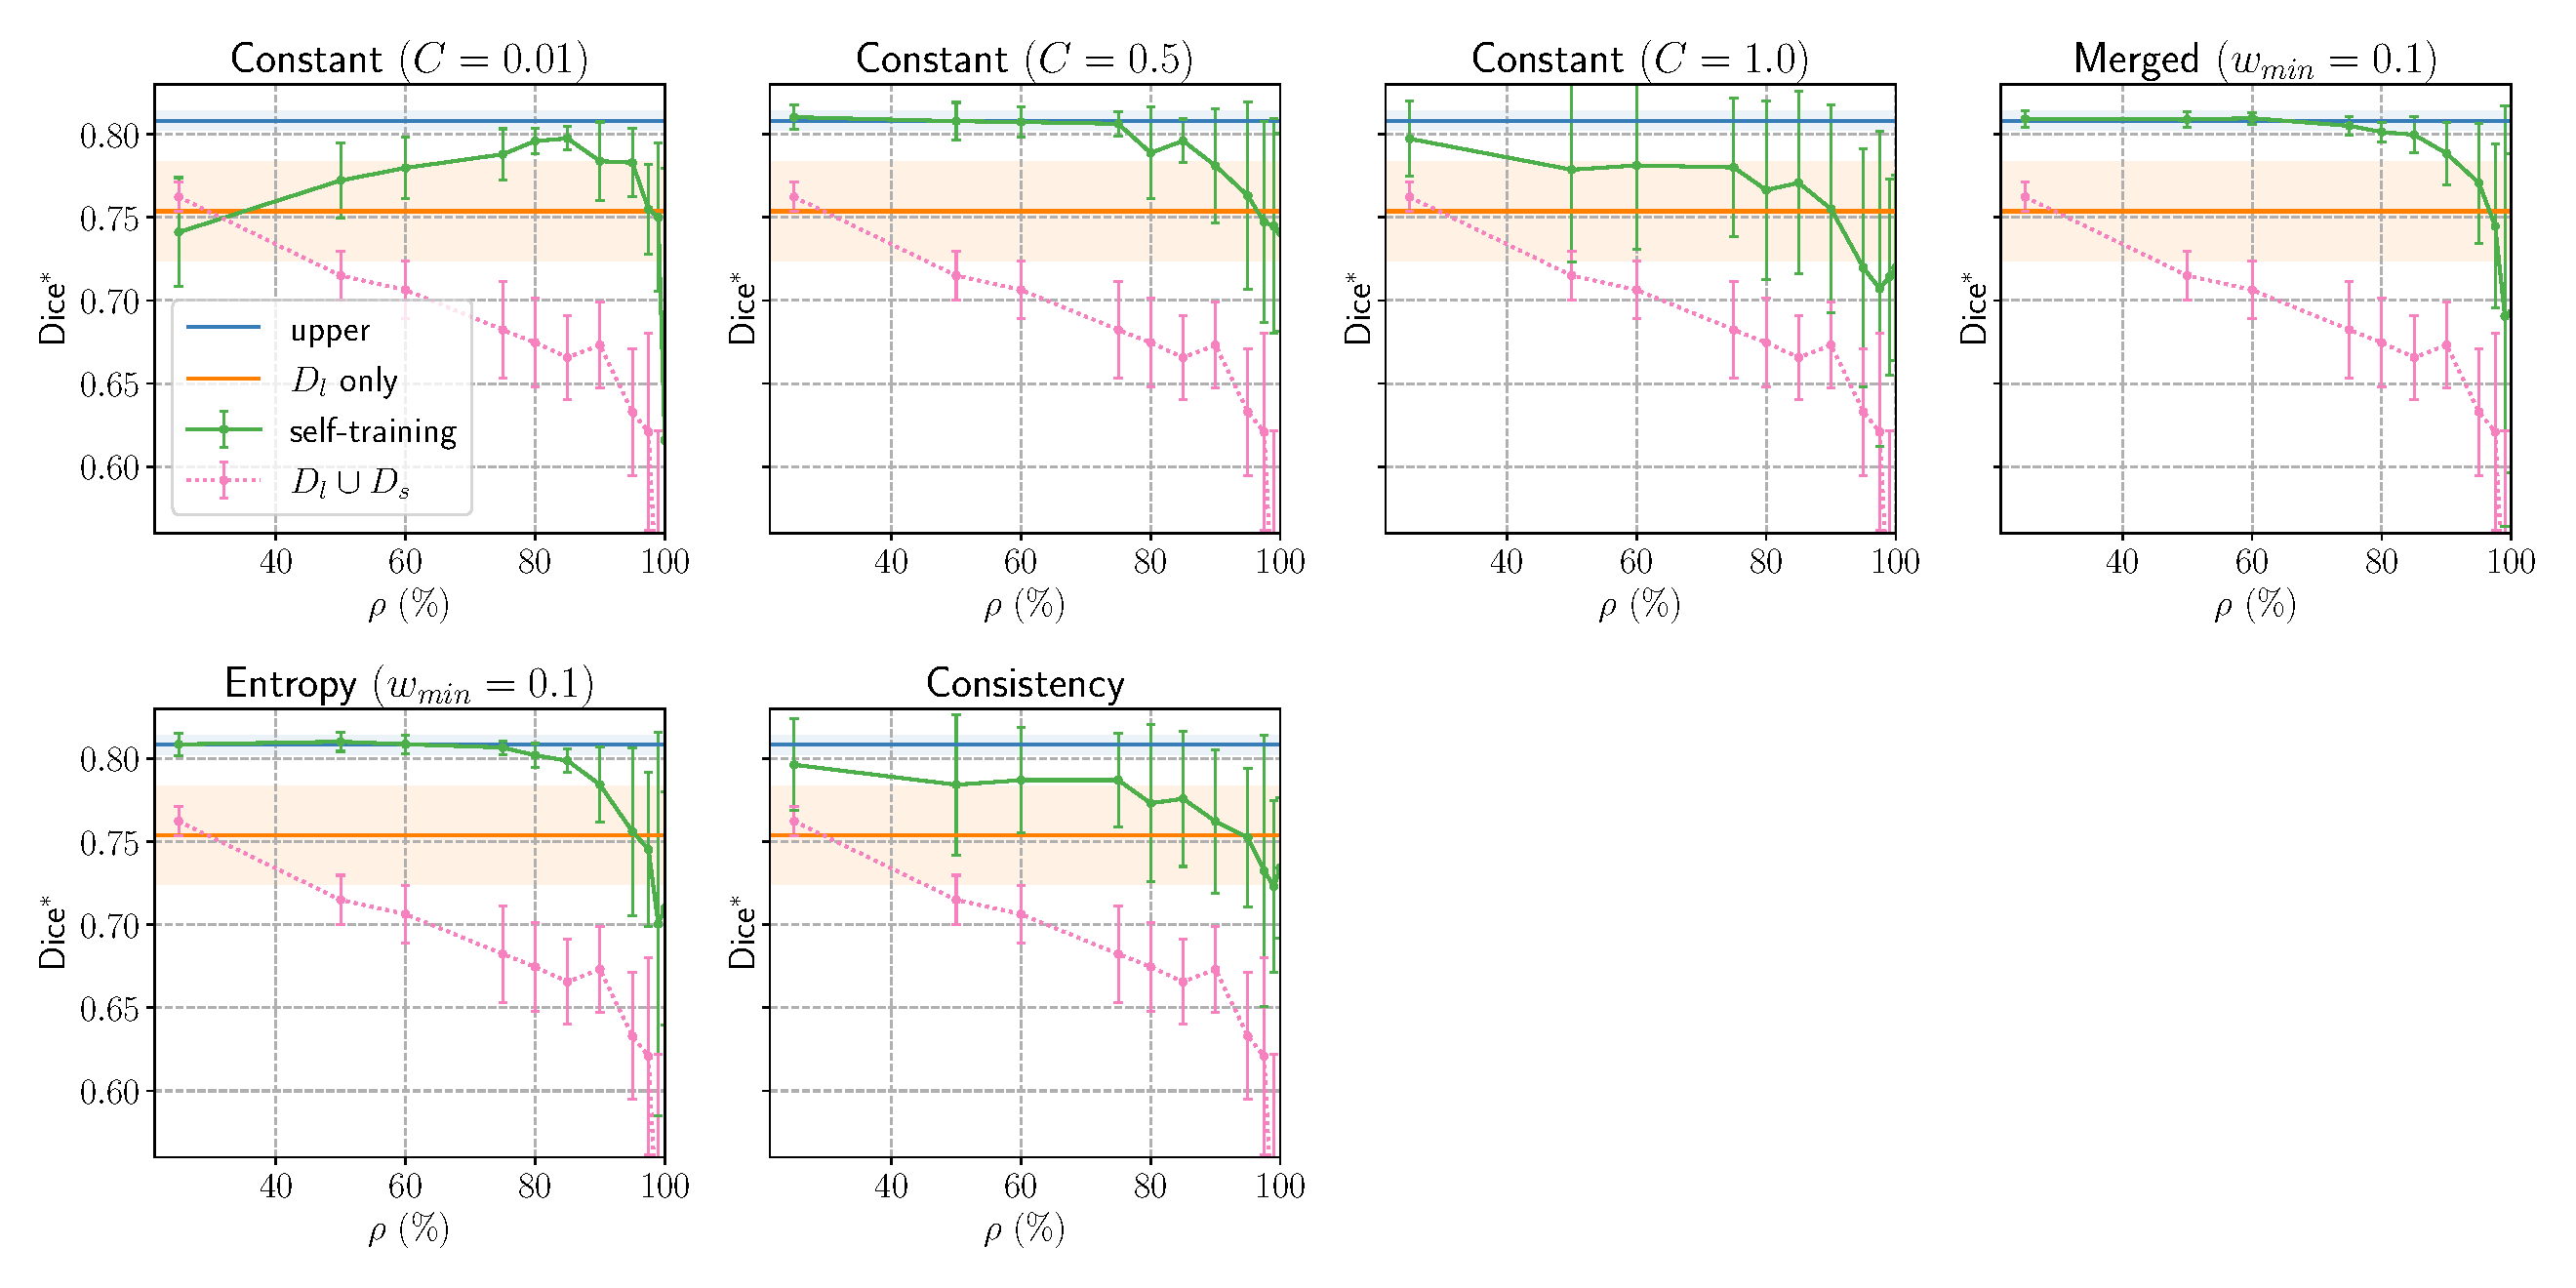
\includegraphics[width=\textwidth]{strain/all_monuseg_test_pxl_self_hard_dice_rho.pdf}
    \caption{\acrshort{monuseg}, see Figure \ref{fig:strain:rho_exp} for explanation.}
      \label{app:strain:fig:rho_exp_monuseg}
\end{figure}

\begin{figure}
    \centering
    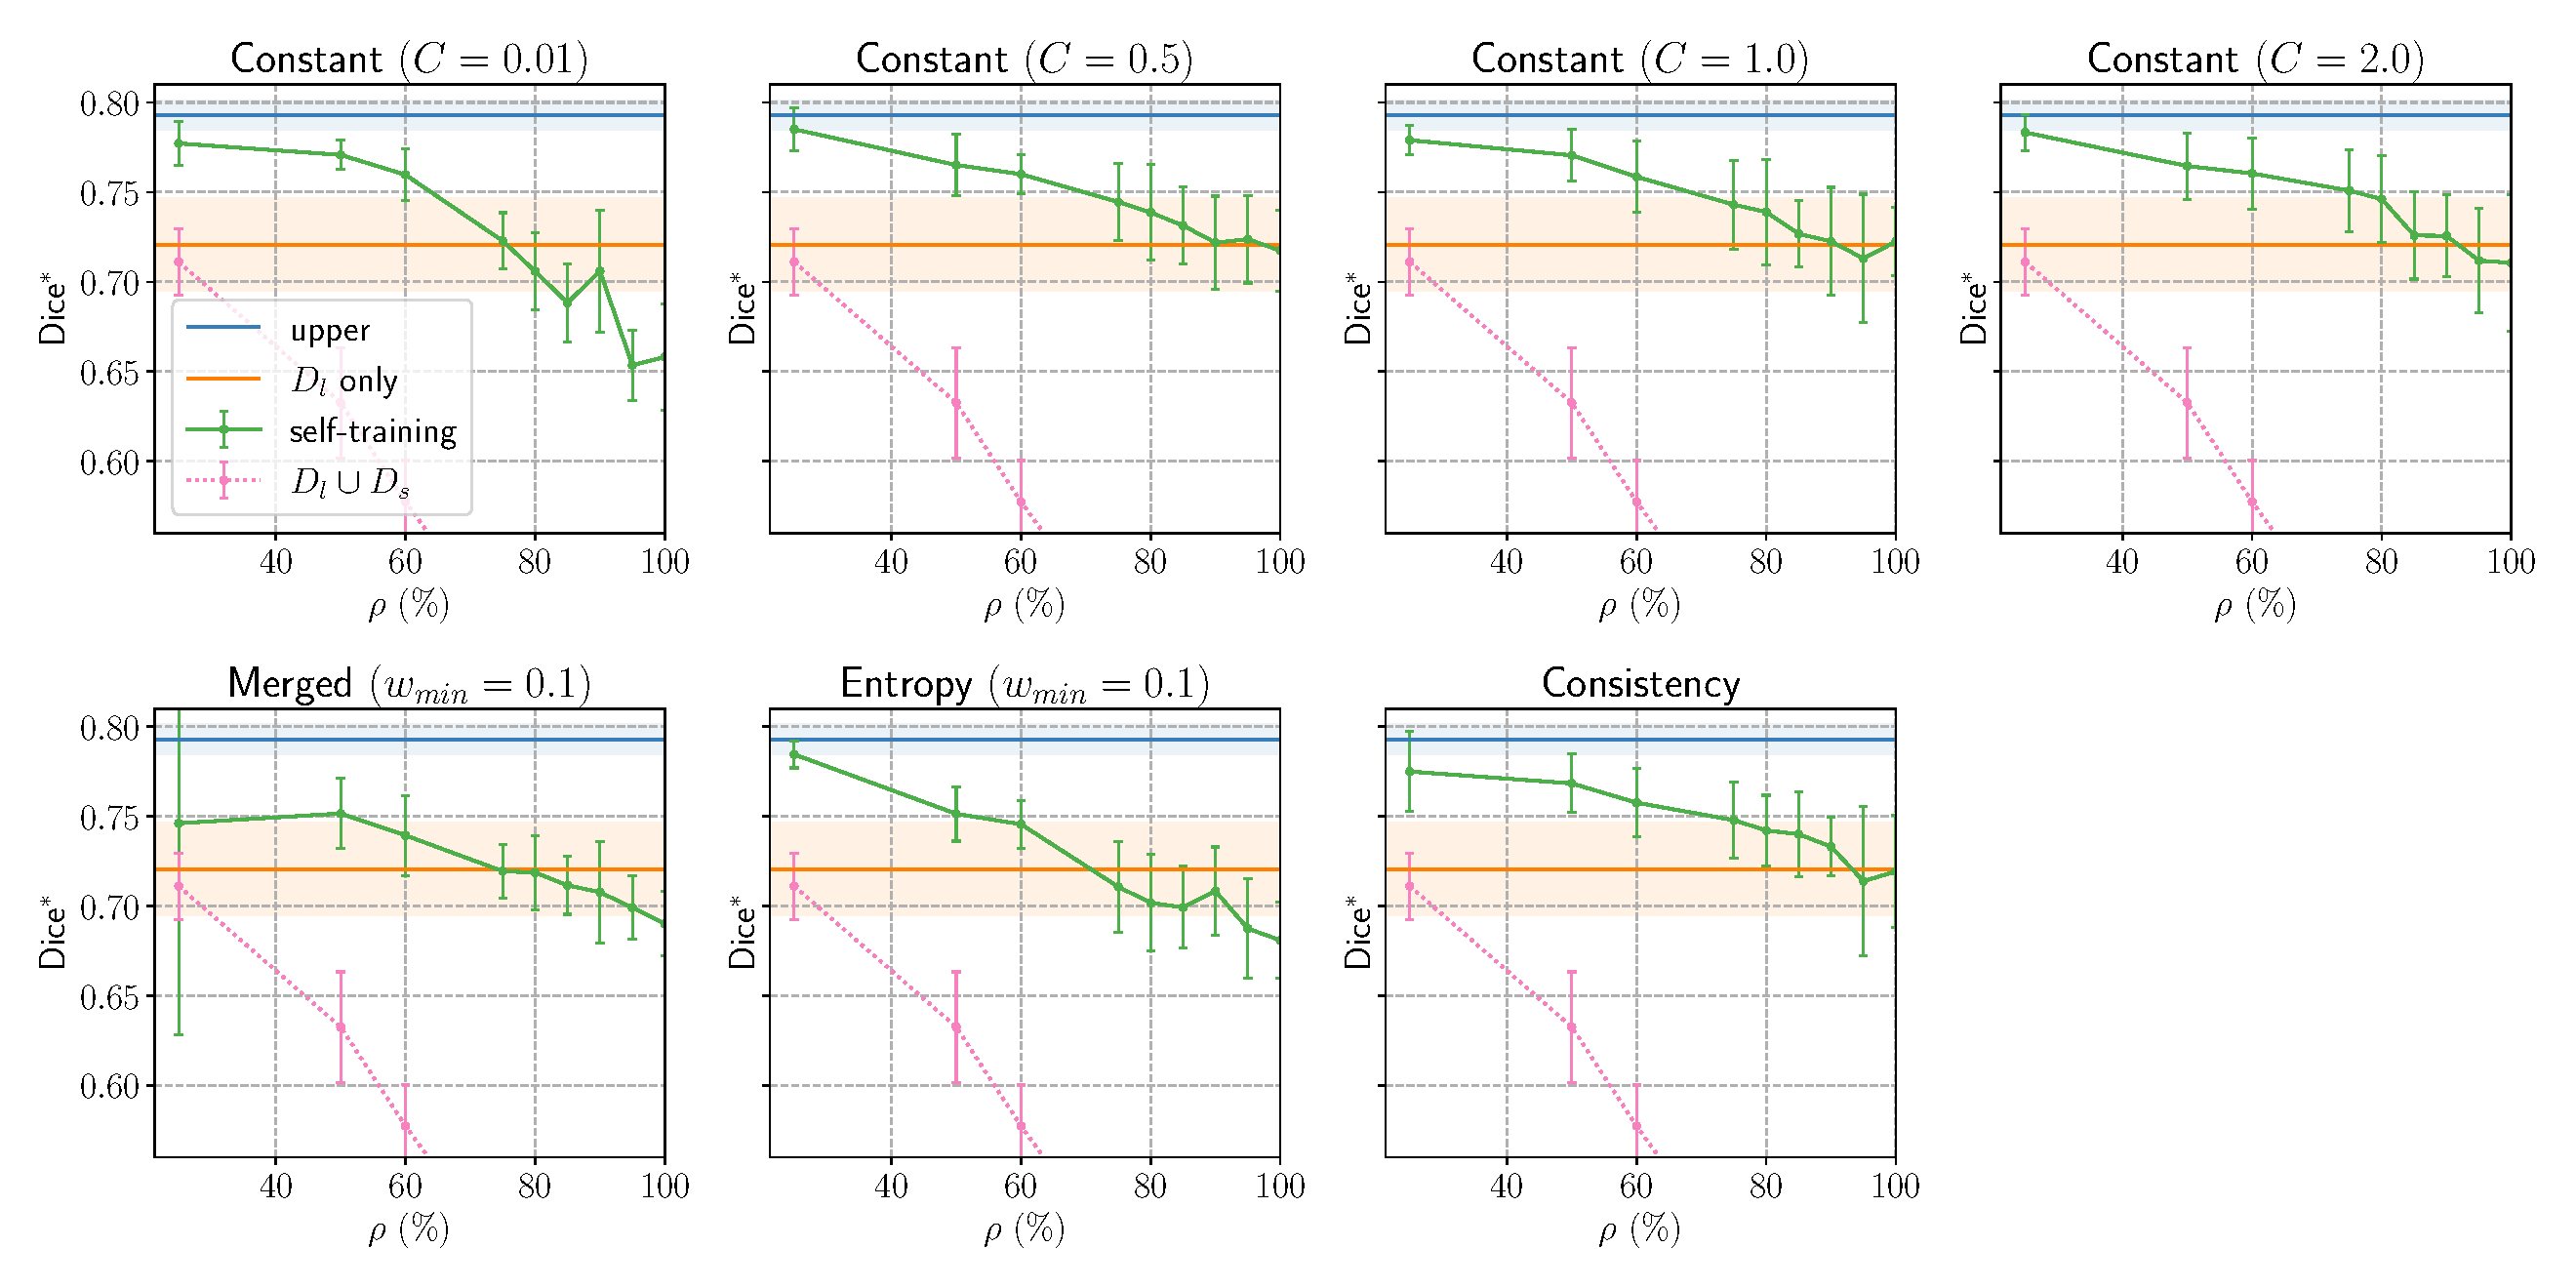
\includegraphics[width=\textwidth]{strain/all_segpc_test_pxl_self_hard_dice_rho.pdf}
    \caption{\acrshort{segpc}, see Figure \ref{fig:strain:rho_exp} for explanation.}
    \label{app:strain:fig:rho_exp_segpc}
\end{figure} 

\begin{figure}
    \centering
    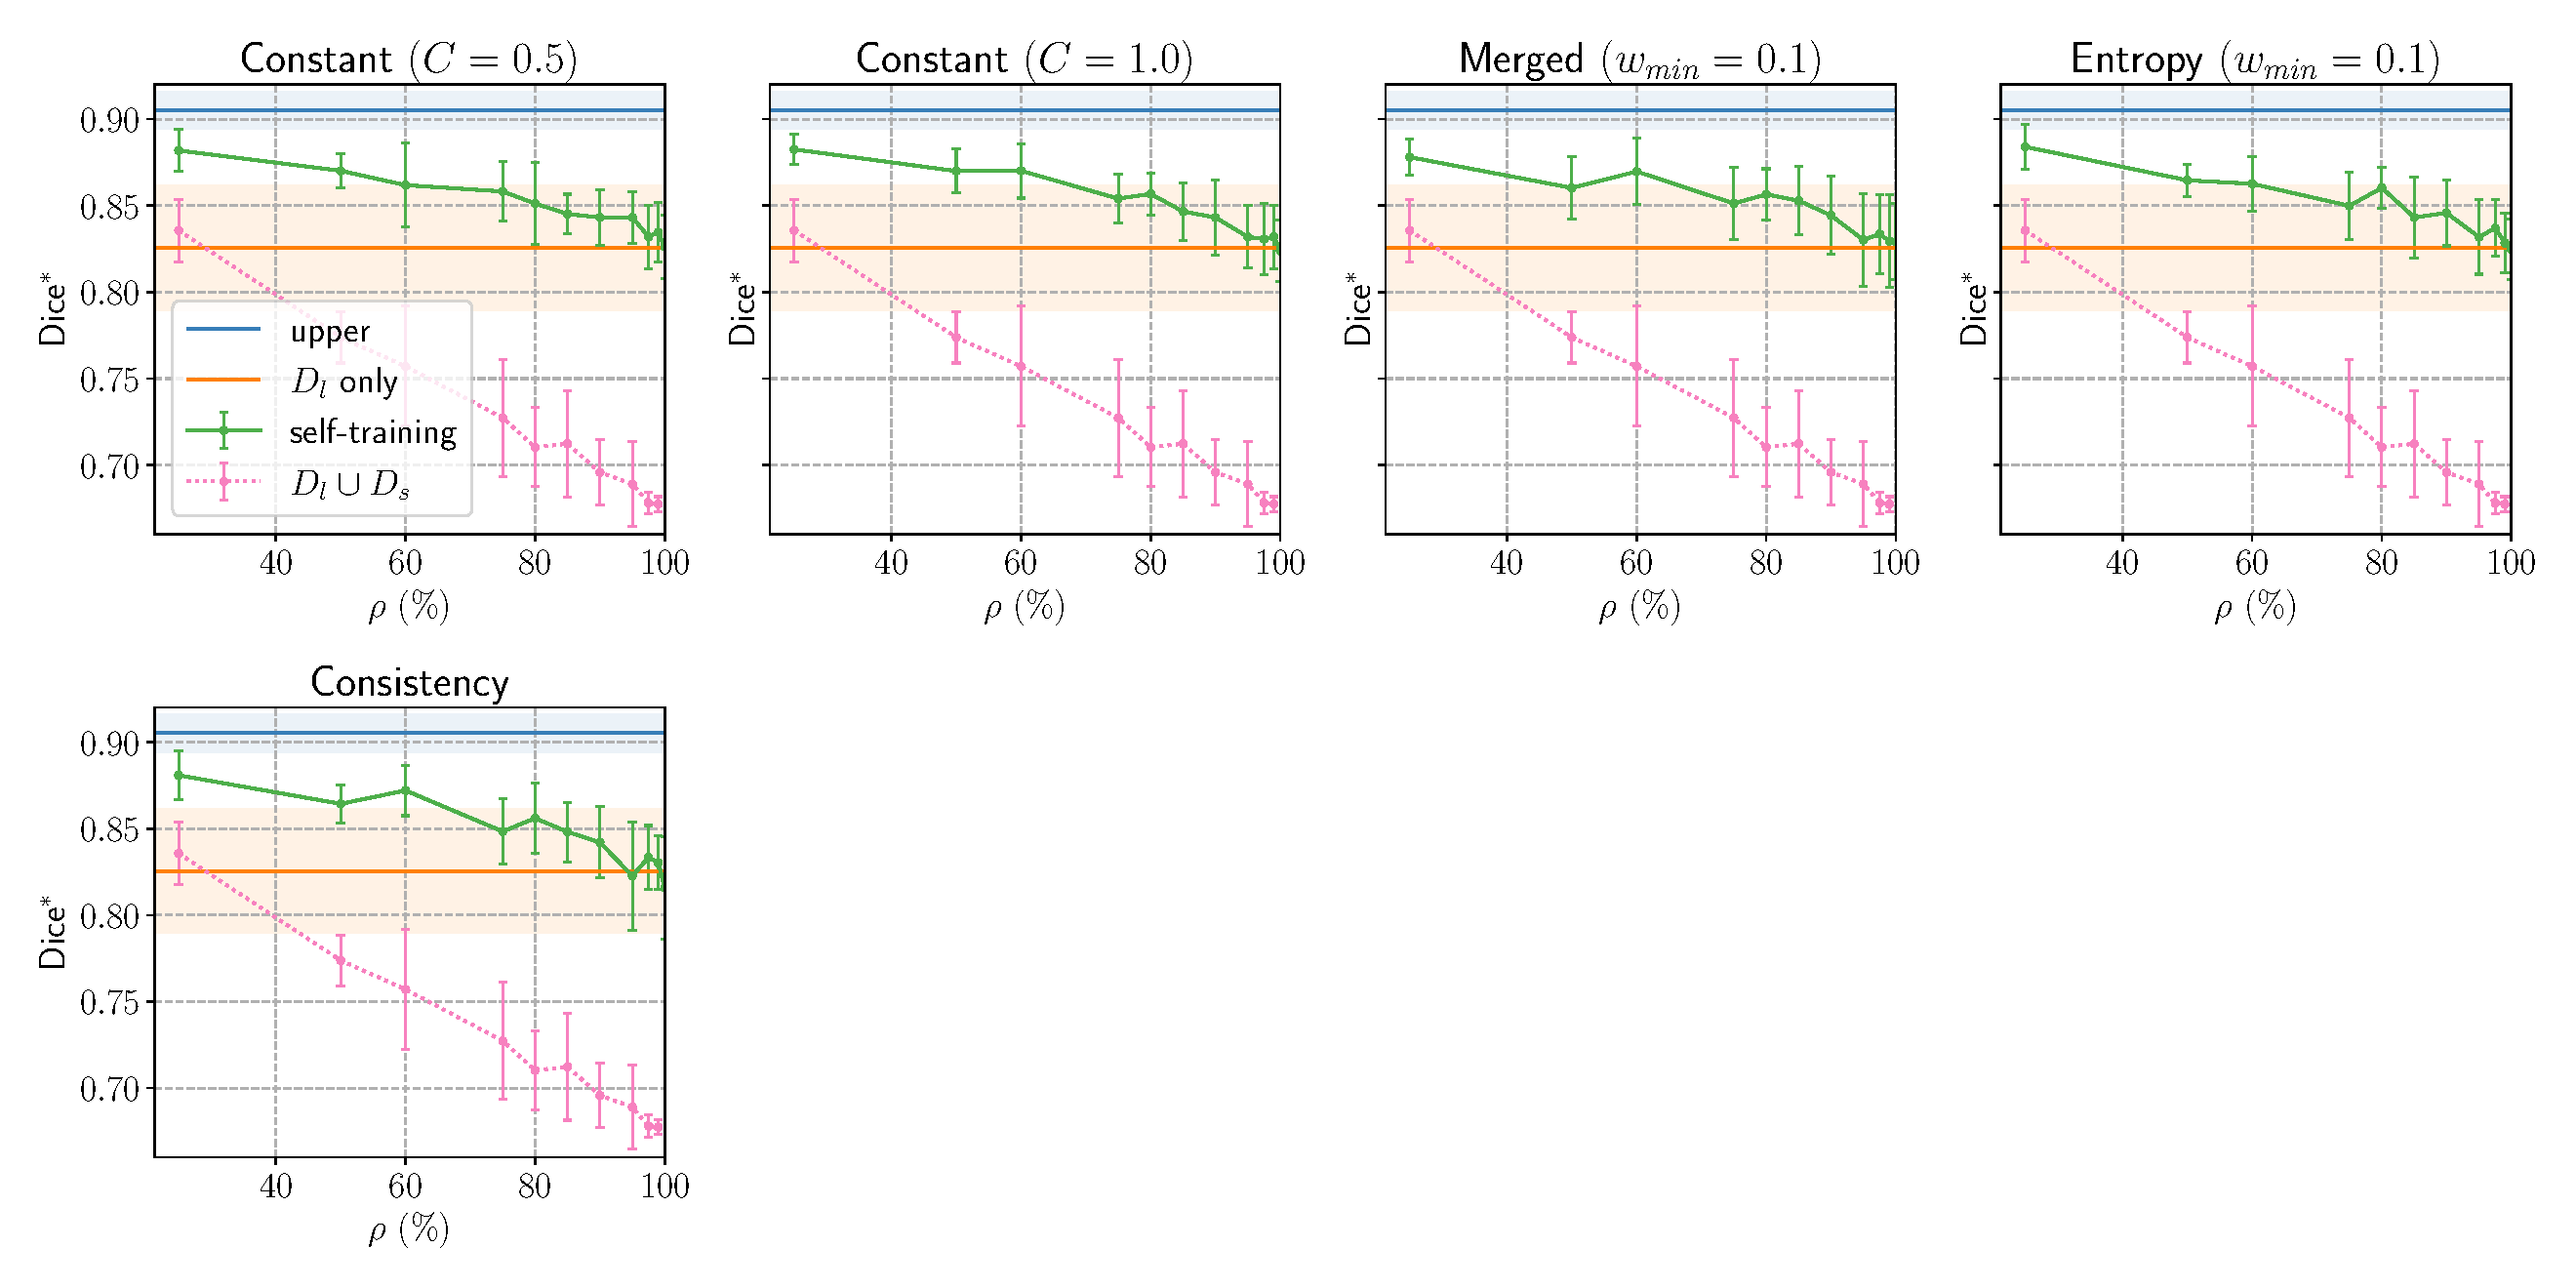
\includegraphics[width=\textwidth]{strain/all_glas_test_pxl_self_hard_dice_rho.pdf}
    \caption{\acrshort{glas}, see Figure \ref{fig:strain:rho_exp} for explanation.}
    \label{app:strain:fig:rho_exp_glas}
\end{figure}
  
\section{The Thyroid \acrshort{fnab} ontology}
\label{app:strain:sec:thyroidontology}

The Thyroid \acrshort{fnab} dataset was labeled by experienced pathologists who followed a detailed ontology to categorize their annotations:

% from the team of Isabelle Salmon from Erasme Hospital in Brussels

\begin{enumerate}
	\item Architectural patterns (see examples in Figure \ref{app:strain:fig:patterns_examples}):
	\begin{itemize}
		\item Normal follicular architectural pattern
		\item Proliferative follicular architectural pattern
		\item Proliferative follicular architectural pattern (minor sign)
	\end{itemize}
	\item Nuclear features (see examples in Figure \ref{app:strain:fig:cells_examples}):
	\begin{itemize}
		\item Papillary cell NOS
		\item Normal follicular cells
		\item Normal follicular cell with pseudo-inclusion (artefact)
		\item Papillary cell with ground glass nuclei
		\item Papillary cell with nuclear grooves
		\item Papillary cell with inclusion
	\end{itemize}
	\item Others:
	\begin{itemize}
		\item Macrophages
		\item Red blood cells
		\item PN (polynuclear)
		\item Colloid
		\item Artefacts
		\item Background
	\end{itemize}
\end{enumerate}

